\textbf{***Mention first Mirrorshades test with single webcam providing small floating window in corner of virtual view (video is on youtube/Mirrorshades repo).}

\textbf{**Show lens comparison picture from blog \& a (new?) screenshot showing FoV of the camera feeds compared to that of Rift \& explain why the discrepancy doesn't matter, especially when the Rift is fully extended.}

\textbf{***This chapter has none of the actual design/development really, it just presents the finished platform.}

%=========================================================================================================
%=========================================================================================================

\subsection{Case Study - St Salvator's Chapel}
Founded in 1450 but internally stripped of its medieval fittings during the Protestant Reformation (1517 - 1648), St Salvator's chapel in St Andrews looks markedly different in the present day than it did upon its completion. An existing VR reconstruction of the chapel as it stood in the period 1450-1460 \& the marked differences between the internal appearance of the VR building \& the current building (including the replacement of the original stone roof with a wooden one \& drastically different dividing of the internal space) make this chapel an ideal candidate within the context of cultural heritage for a mobile XR system to be applied. Figure \ref{sallies_layout} shows the 1450-1460 layout of the chapel (including the paths that the IPS has been prepared upon).

\begin{figure}[h]
	\begin{center}
		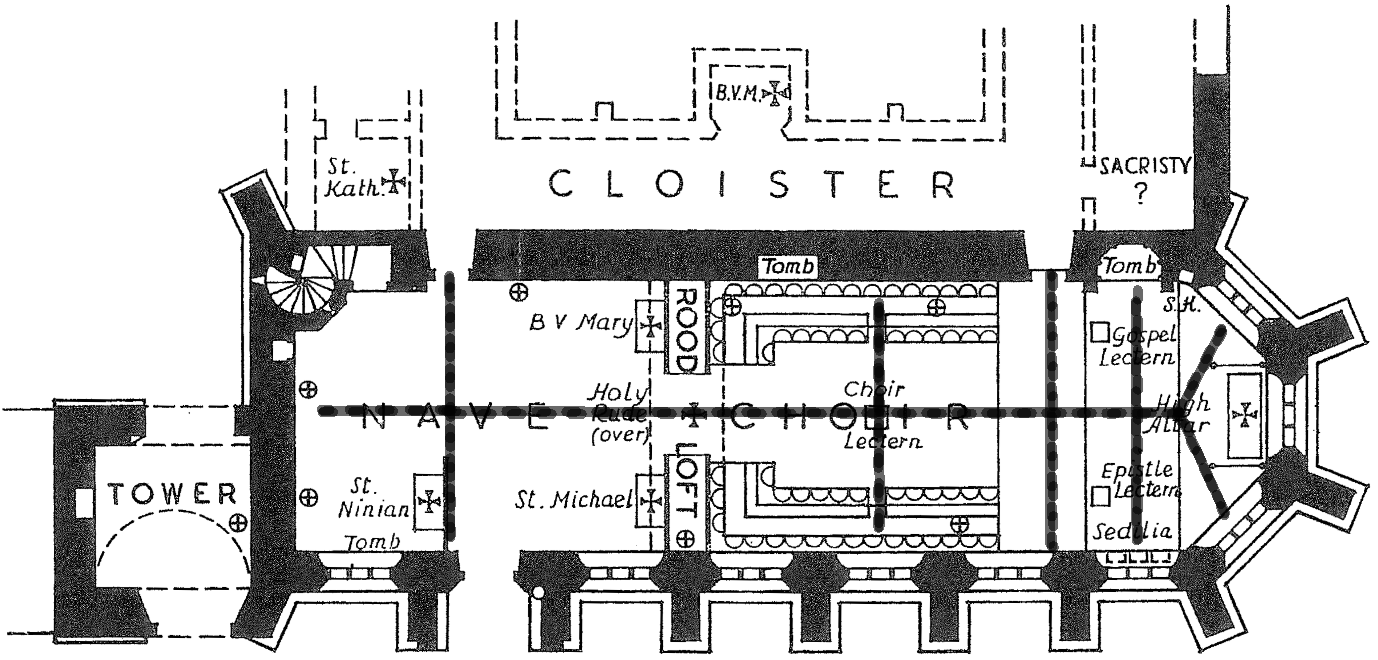
\includegraphics[width=0.7\textwidth]{images/sallies_layout.png}
		\caption{Floor plan of St Salvator's chapel, with IPS routes.}
		\label{sallies_layout}
	\end{center}
\end{figure}

\clearpage

%=========================================================================================================
%=========================================================================================================

\section{The Mirrorshades Platform}
Figure \ref{systemarchitecture} presents a high level architectural overview of our mobile XR platform, dubbed Mirrorshades\footnote{\textbf{Mirrorshades: The Cyberpunk Anthology} (1986) is a defining cyberpunk short story collection, edited by Bruce Sterling.}.

\begin{figure}[h]
	\thispagestyle{empty}
	\begin{center}
		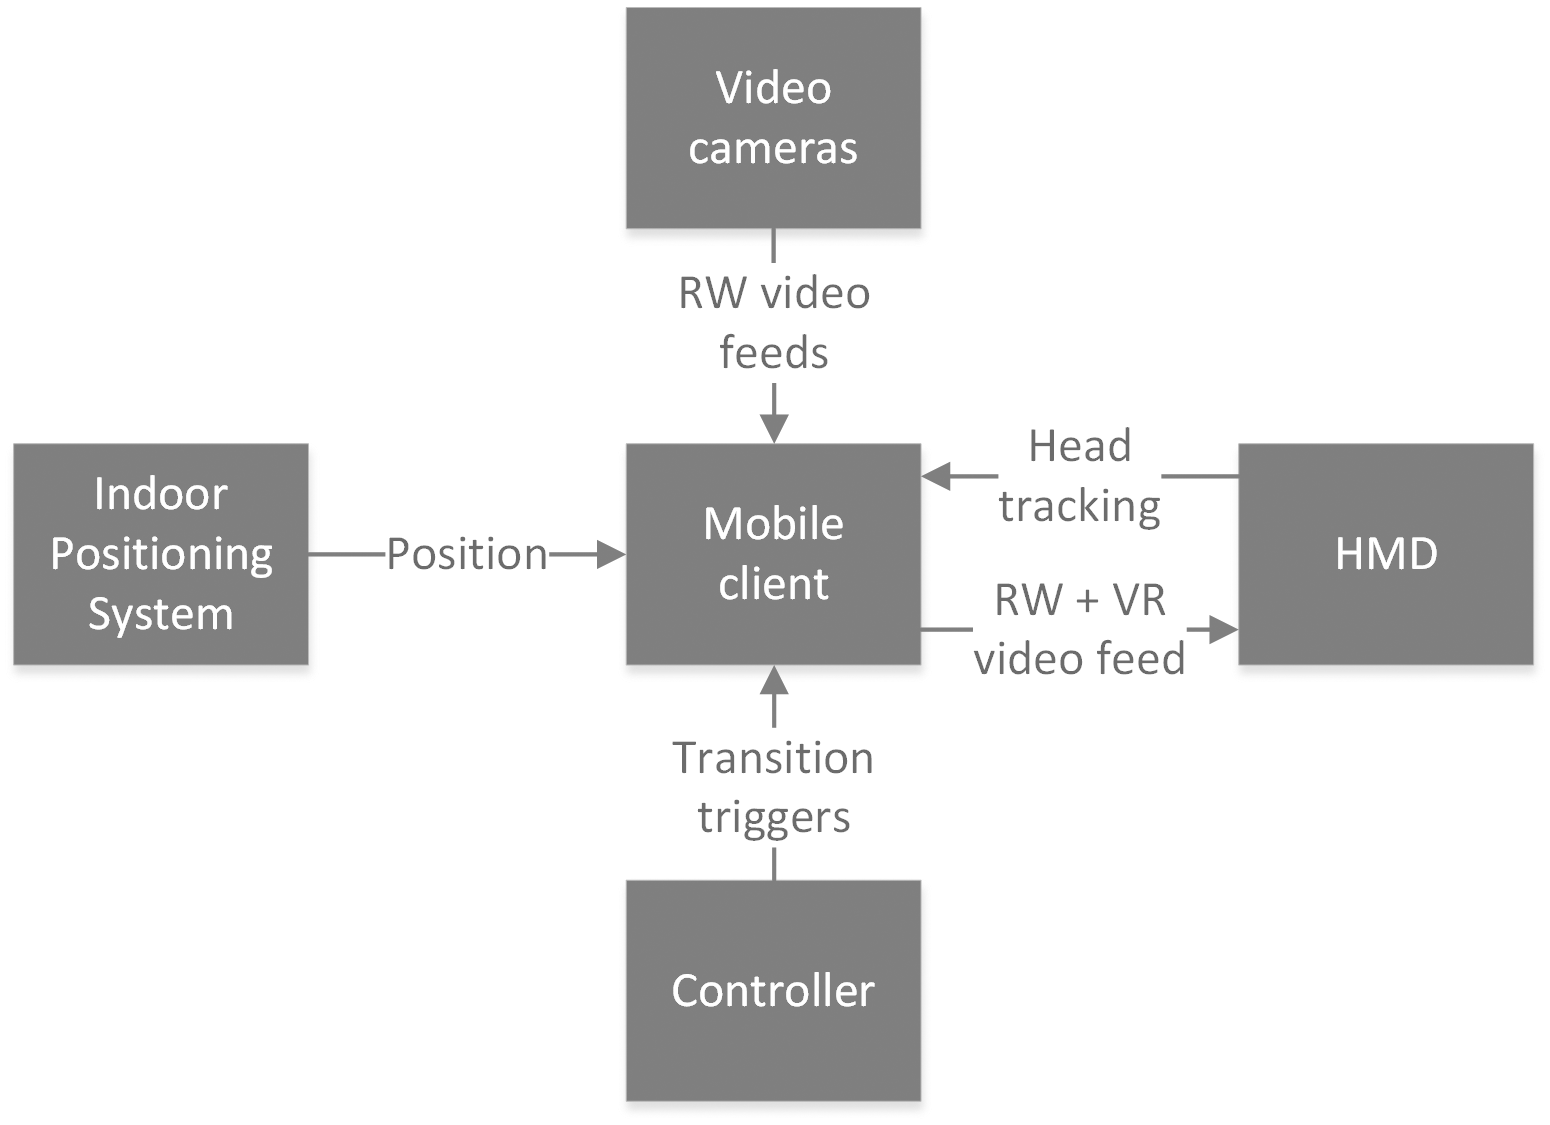
\includegraphics[width=.5\linewidth]{images/system-architecture.png}
		\caption{Overview of the Mirrorshades platform.}
		\label{systemarchitecture}
	\end{center}
\end{figure}

%=========================================================================================================
%=========================================================================================================

\subsection{Implementation}
Figure \ref{experimentalimplementation} presents an overview of the implementation of the Mirrorshades platform design for use in the chapel investigations.

\begin{figure}[h]
	\thispagestyle{empty}
	\begin{center}
		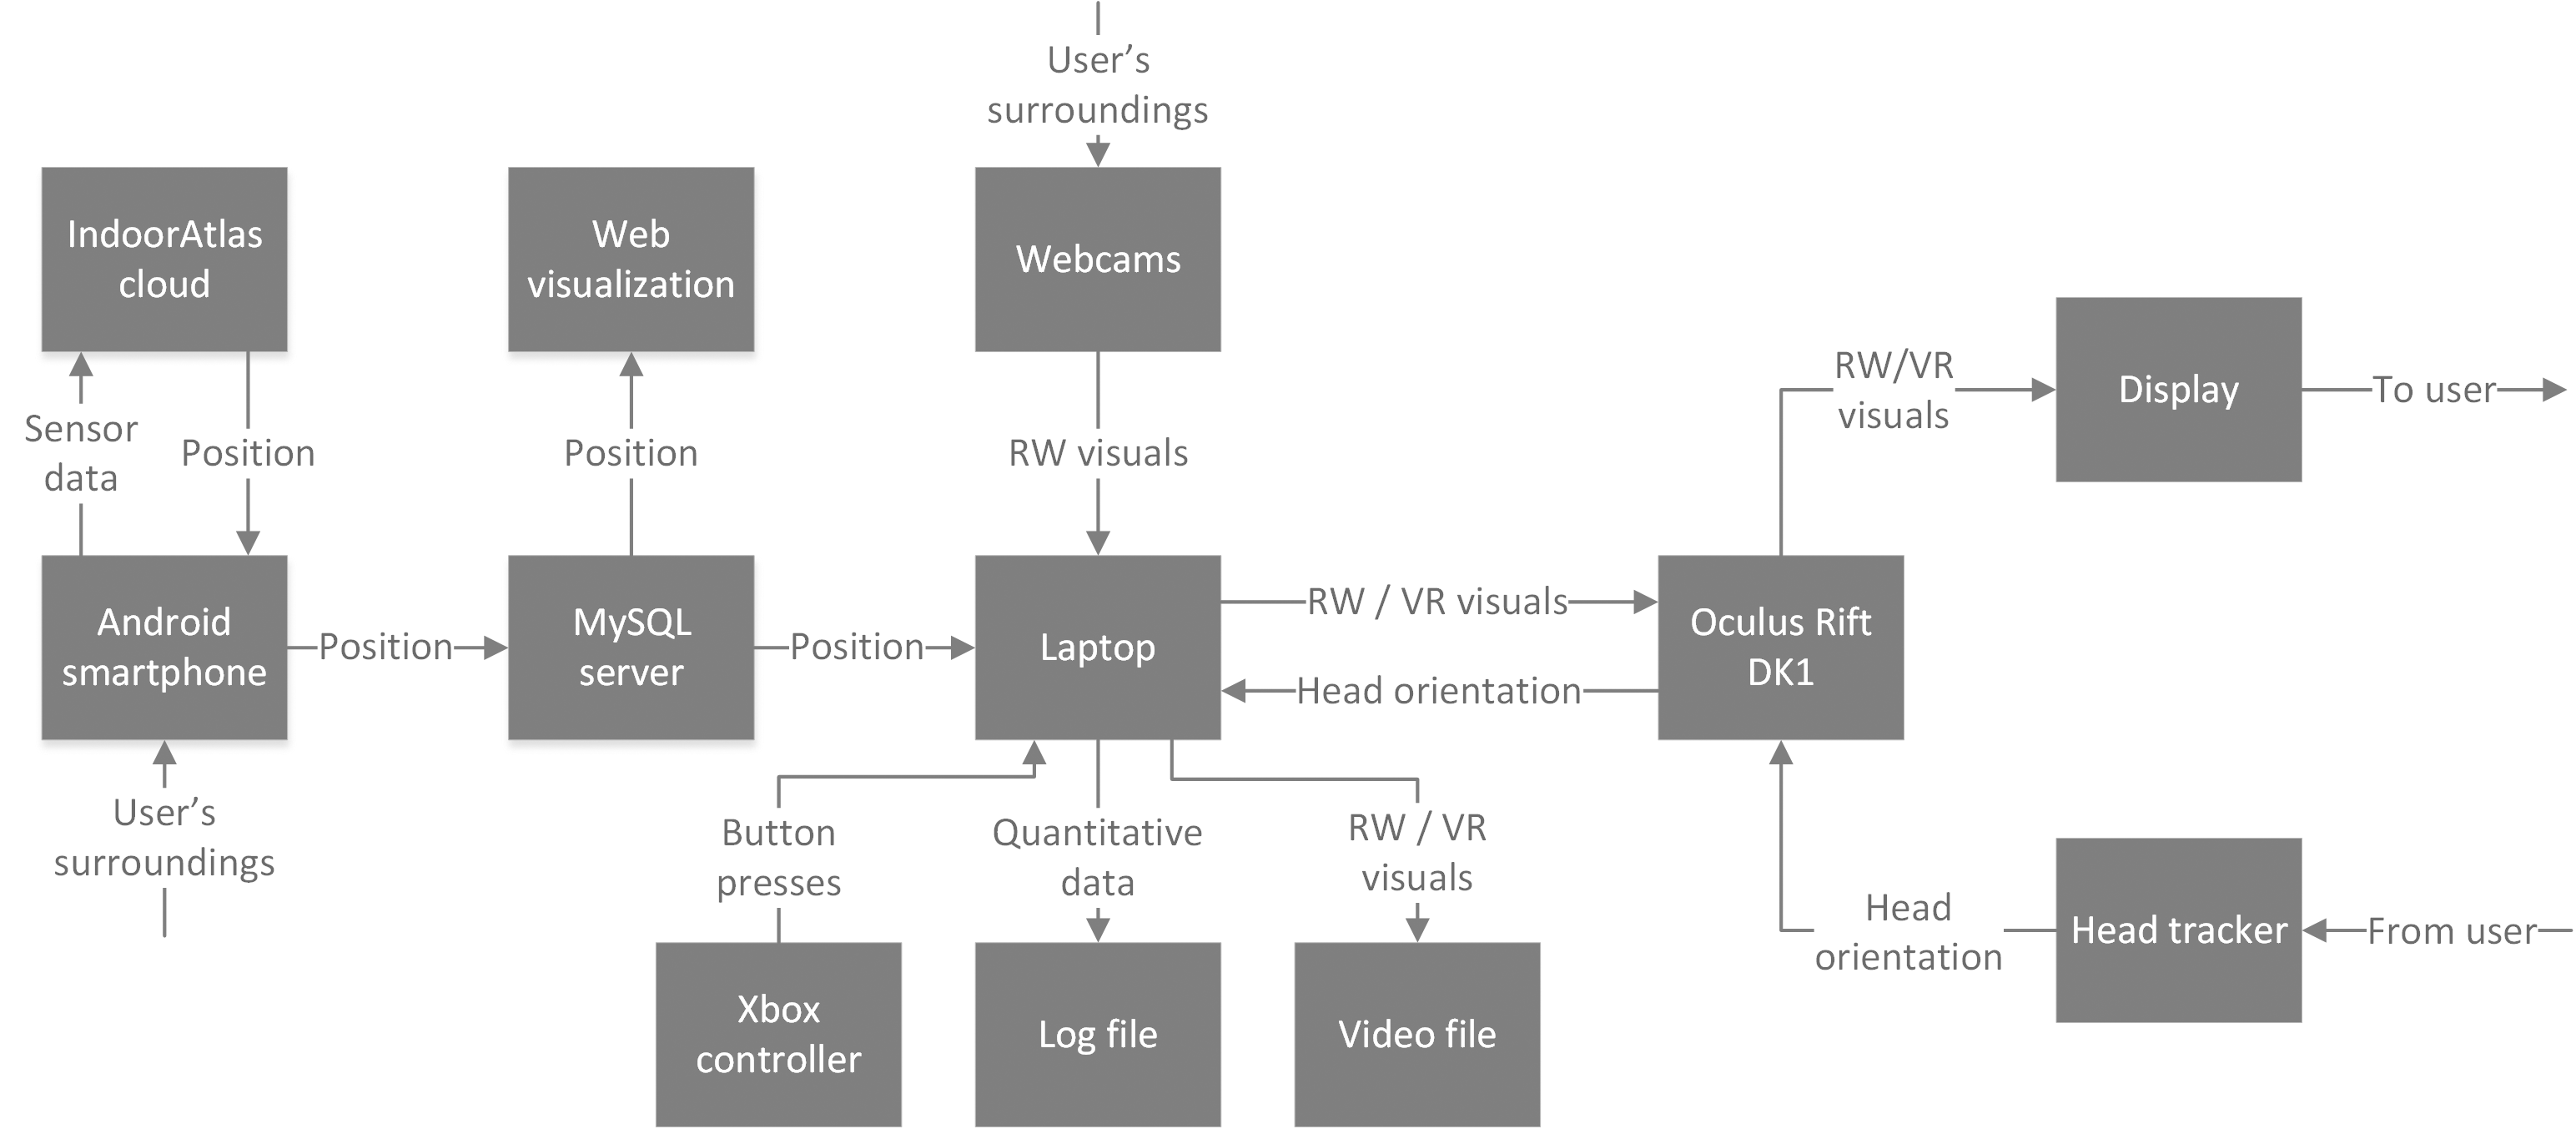
\includegraphics[width=.925\linewidth]{images/experimental-implementation.png}
		\caption{Implementation of Mirrorshades platform.}
		\label{experimentalimplementation}
	\end{center}
\end{figure}

\subsection{Hardware Components}
The hardware of the implementation comprises;

\begin{itemize}
	\item an Oculus Rift DK1 HMD, including a 9-axis (3dof rotational) head tracker sampling at 1000Hz \& mounted with a stereo camera solution comprising 2x Logitech C310 webcams modified with M12 lens mounts \& 2.1mm lenses to provide approximately 87 degrees horizontal FOV of the RW environment (see figure \ref{rift});
	\item a USB battery pack, to power the HMD;
	\item a small laptop computer, with an Intel i7-3632QM processor, Nvidia GT 650M graphics card \& 16GiB system memory;
	\item an Android smartphone, running Android 4.4.4;
	\item an Xbox 360 wireless controller, with USB receiver.
\end{itemize}

\begin{figure}[h]
	\begin{center}
		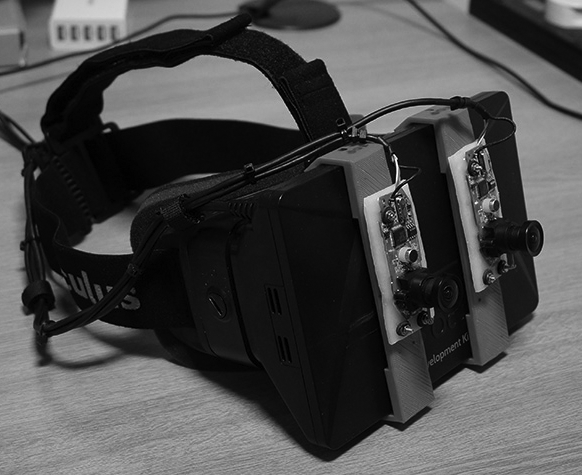
\includegraphics[width=0.6\textwidth]{images/rift.png}
		\caption{HMD with stereo camera solution.}
		\label{rift}
	\end{center}
\end{figure}

\subsection{Software Components}
The software of the implementation comprises;

\begin{itemize}
	\item an Android application that runs on the smartphone, determines the location of the phone within the building that it is in using the IndoorAtlas IPS~\cite{IndoorAtlasLtd.2012} (figure \ref{sallies_layout} shows the paths within the chapel upon which the IPS has been configured) \& submits these location data via PHP to a database server;
	\item a MySQL database server that stores location data for the phone \& allows these data to be accessed both by the Unity application running upon the laptop \& by a web visualisation;
	\item a Unity application that runs on the laptop.
\end{itemize}

\subsection{Integration of Components}
The Unity application hosts the VR representation of the chapel \& takes in feeds from both webcams, the HMD head tracker \& the Xbox controller. It also polls the database server for the most recent position data. All of these inputs are combined together to form the visual output for the HMD to display to the user.

As the user moves their head, the visuals that are presented to them upon the HMD's display change accordingly; the RW visuals change due to the webcams being physically fixed to the HMD \& the VR visuals change due to data from the head tracker being used to change the orientation of the in game `cameras' accordingly.

As the user changes their position by walking, the visuals that are presented to them upon the HMD's display also change accordingly; again the RW visuals change due to the webcams' position upon the HMD whilst the VR visuals change due to the user's position, as reported by the smartphone \& the IndoorAtlas solution, being used to move the position of the in game cameras to the equivalent position within the VR representation.

As the user presses buttons or pulls triggers upon the Xbox controller, the visuals that are presented to them upon the HMD's display transition between RW \& VR in different styles depending upon which button/trigger was activated.

%=========================================================================================================
%=========================================================================================================

\section{Investigation 1 - The Case for Mobile XR}
\label{investigation1}
This first investigation will compare interaction with the RW \& VR chapel using Mirrorshades to interaction with the same content separately, the latter being the approach usually adopted for dissemination of VR content in cultural heritage contexts. Participants will complete a task that will promote active comparison \& contrast of the RW \& VR environments, whilst navigating a set route. This investigation will gauge through experimentation whether the Mirrorshades platform provides any value over the traditional manner in which the same VR content might be disseminated at a cultural heritage site.

%spatial \& temporal separation

\subsection{Setting \& Task}
This investigation comprises two phases;

\begin{enumerate}
	\item Participants will experience the RW \& VR chapels separately. They will navigate the VR chapel from a stationary position, as one might expect to see a VR installation at a cultural heritage site, using the Xbox controller to move around the VR environment observed via the HMD. The HMD will obscure their view of the RW chapel around them. Subsequently, they will navigate the RW chapel without the HMD or any associated equipment.
	\item Participants will experience the RW \& VR chapels in tandem using the Mirrorshades platform. They will wear the HMD, holding the Xbox controller in their right hand \& the smartphone in their left, with the laptop \& battery pack in a satchel worn over one shoulder. One style of transition will be available to the participants during this phase.
\end{enumerate}

In all 3 scenarios (phase 1 VR, phase 1 RW, phase 2 RW + VR) the participant will navigate the same route \& will be instructed to identify a particular feature/object within the chapel (see figures \ref{pews} \& \ref{ceiling}), situated somewhere upon the set route, that differs in its appearance \&/or location between the RW \& VR chapels. The order in which the two phases are completed will be randomised between participants, as will the features that they are told to observe in each phase. Participants will have a maximum length of time to navigate the route \& will be allowed to stop before this time has elapsed should they wish.

%\begin{figure}[h]
%	\begin{center}
%		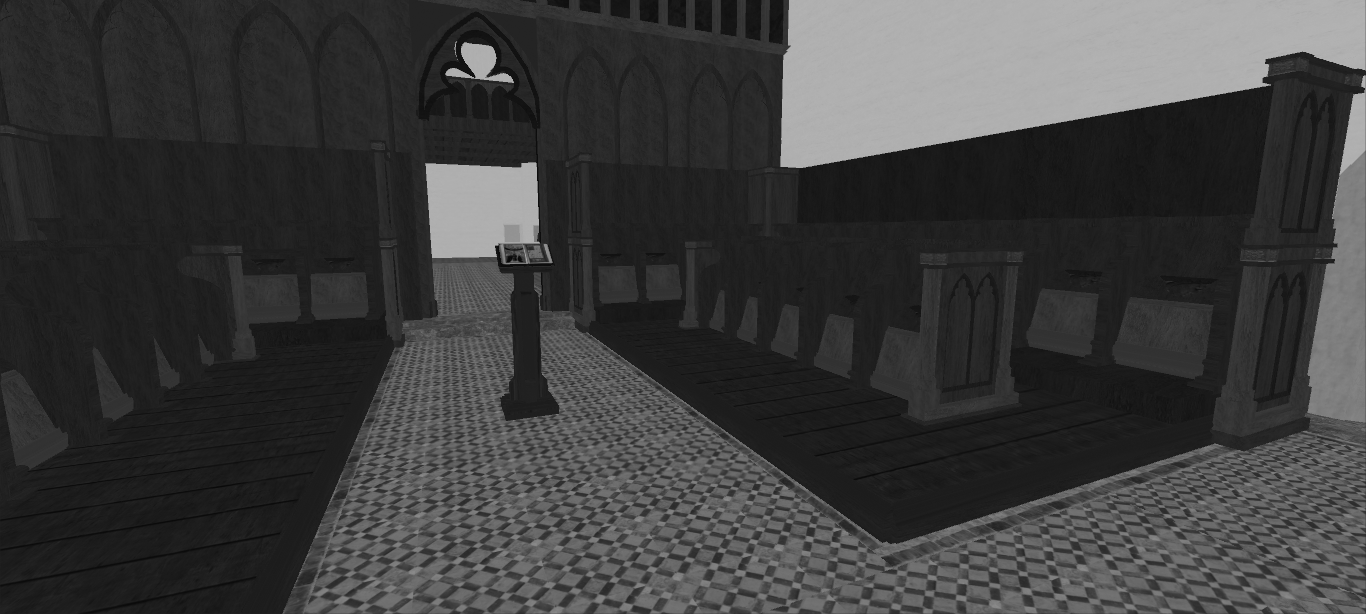
\includegraphics[width=0.7\textwidth]{images/pews.png}
%		\caption{Chapel pews, greater in number in present day.}
%		\label{pews}
%	\end{center}	
%\end{figure}

%\begin{figure}[h]
%	\begin{center}
%		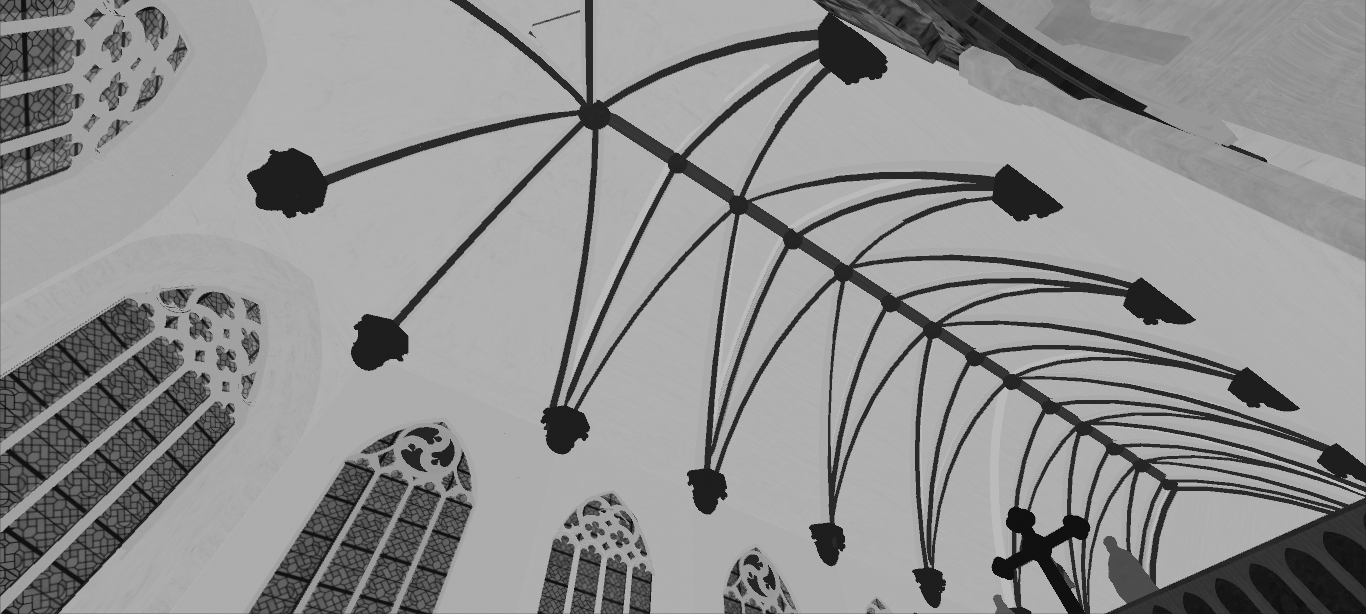
\includegraphics[width=0.7\textwidth]{images/ceiling.png}
%		\caption{Chapel ceiling, different construction in present day.}
%		\label{ceiling}
%	\end{center}	
%\end{figure}

%\begin{figure}[h]
%	\begin{center}
%		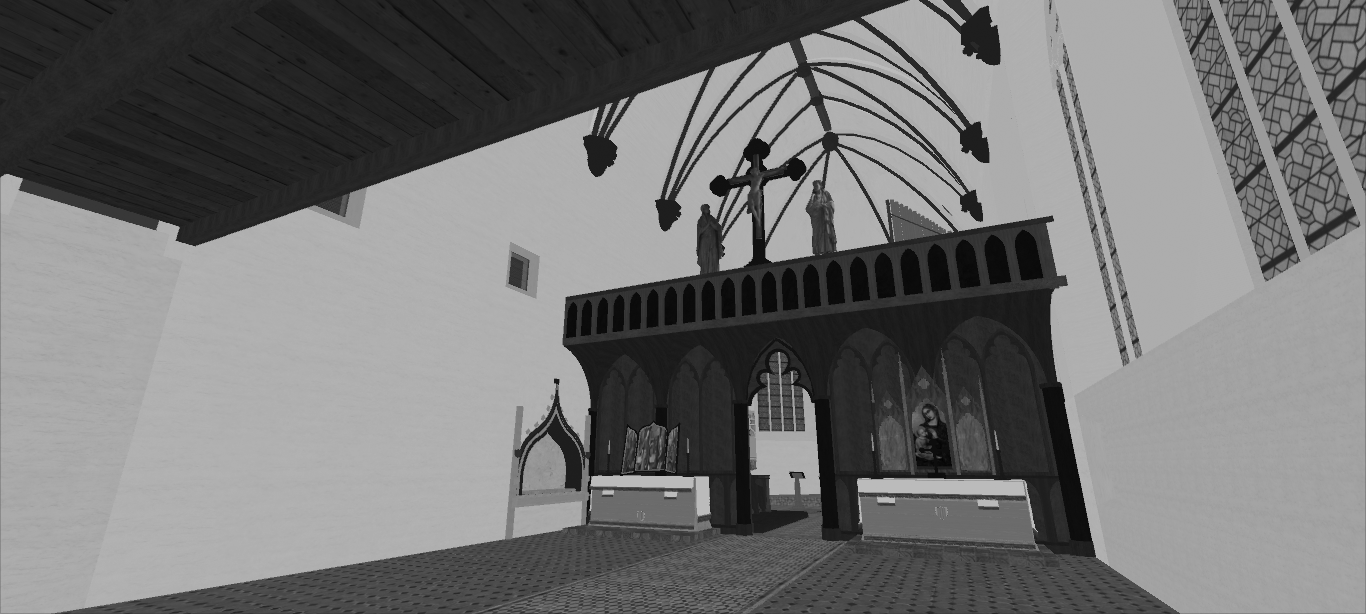
\includegraphics[width=0.7\textwidth]{images/division.png}
%		\caption{Division of the internal space of the chapel, different position in present day.}
%		\label{division}
%	\end{center}	
%\end{figure}

%rows/number of pews
%position of dividing wall
%colour/construction of ceiling
%number/position of lecterns

\subsection{Evaluation Techniques}
Evaluation will be performed via a short structured interview \& completion of the System Usability Scale (SUS)~\cite{Brooke1996}.

%\begin{itemize}
%	\item (General) Which did you prefer?
%	\item Which did you think made it easier for you to perform comparisons between real \& virtual?
%	\item Which was more rewarding (if you were visiting the site genuinely)?
%	\item Which gave a better understanding of the changes that have been effected to the building?
%	\item Did you notice/discover anything in one scenario that you didn't in the other?
%	\item Etc.
%\end{itemize}

\subsection{Hypothesis}
SUS responses are expected to average fairly low due to the cumbersome nature of the platform's implementation. Participants who are able to overcome this cumbersomeness are expected to respond favourably to the platform, with those who cannot overcome it responding in favour of the traditional `separate' approach instead.

%=========================================================================================================
%=========================================================================================================

\subsection{Transition Methods}
Attending to visual stimuli from the RW environment via the webcams is required for the user to safely move around. Delay in the IPS reporting their position \& inaccuracies in these position data (see figure \ref{jack-cole-splodges} for a set of example position data) mean that moving around while attending only to visual stimuli from the VR environment would not be safe for the user, even with unchanging RW obstacles with perfectly accurate representations in the VR environment. Furthermore it is actually likely that RW obstacles will not have equivalent VR representations, such as in a scenario where XR is used to compare \& contrast changes to a building's interior over extended periods of time (such as with the chapel investigations).

\begin{figure}[h]
	\begin{center}
		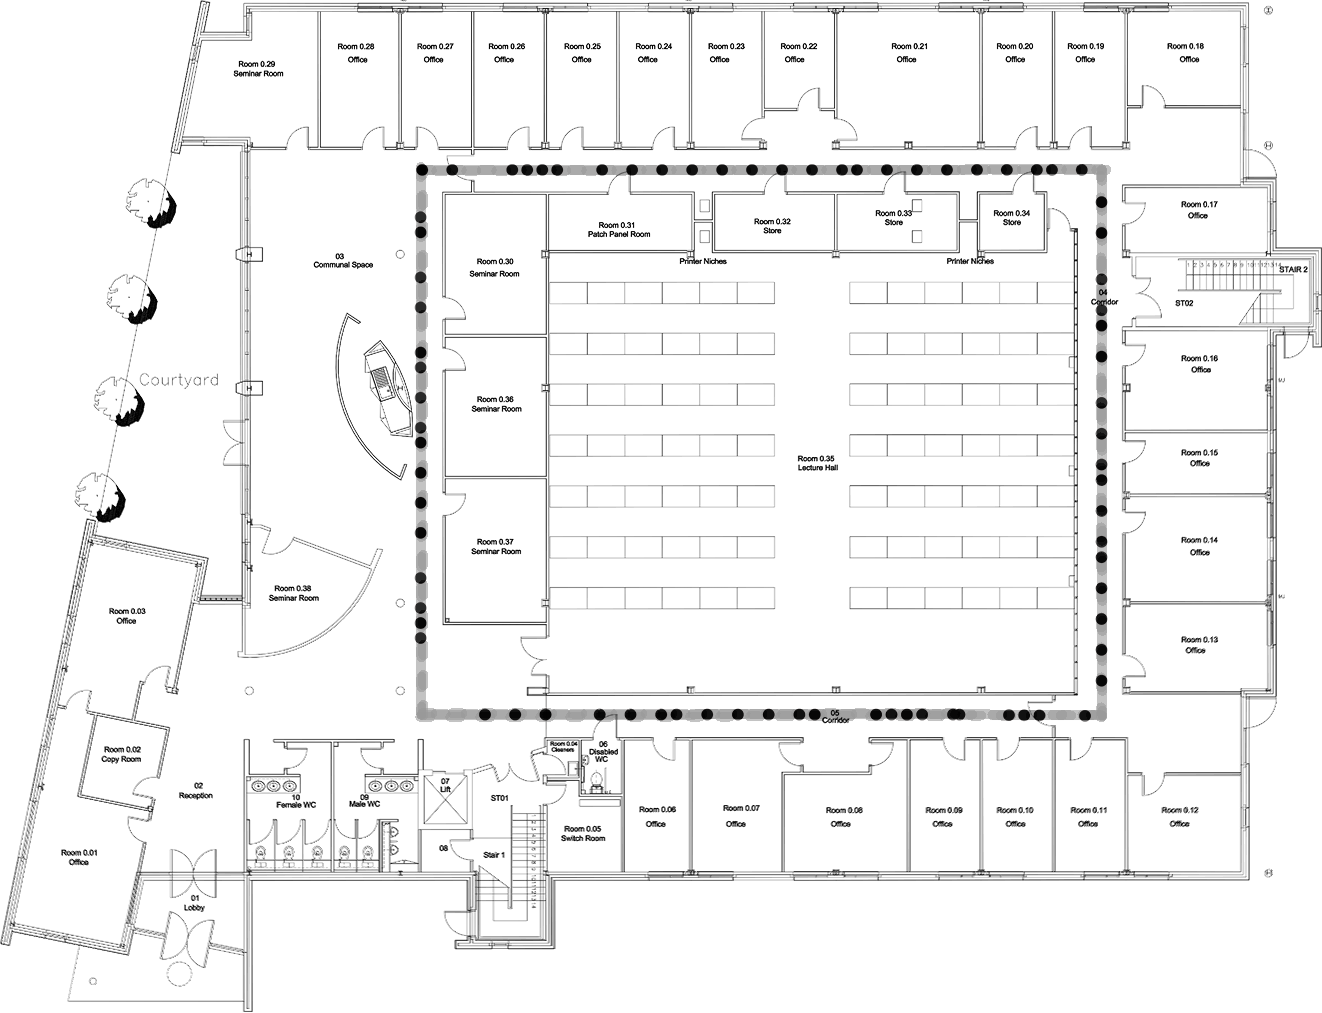
\includegraphics[width=0.7\textwidth]{images/jack-cole-splodges-black.png}
		\caption{Positions (black circles) reported whilst walking a slow lap ($<1$ms$^{-1}$, following gray path) of a departmental building. The building is approximately 40m wide by 30m tall.}
		\label{jack-cole-splodges}
	\end{center}
\end{figure}

Thus the HMD displays the feeds from the webcams as default \& the user must trigger transitions to view the VR environment by pressing a button or pulling a trigger on the controller. Releasing the button/trigger causes the webcam feeds to be displayed again.

\clearpage

\subsubsection{Hard switch}
\label{sub-hardswitch}
The user presses \& holds the \texttt{[A]} button on the controller to switch the visual stimuli displayed by the HMD from RW to VR. When the \texttt{[A]} button is released, the visual stimuli displayed by the HMD switch back from VR to RW. This is a `hard' or `immediate' switch with no fading or transition effect. Figure \ref{scenario1} illustrates this scenario.

\begin{figure}[h]
	\begin{center}
		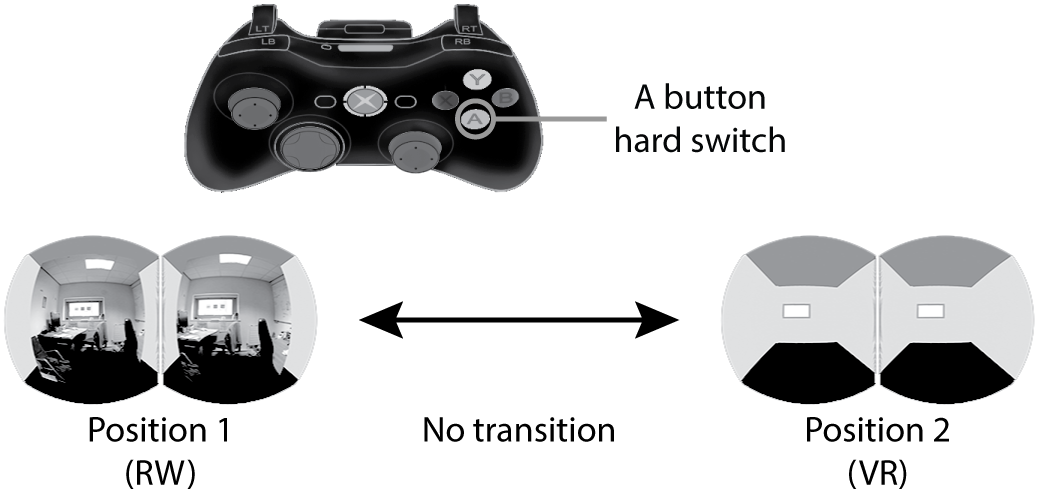
\includegraphics[width=0.7\textwidth]{images/switching-hard-with-controller.png}
		\caption{Hard switch.}
		\label{scenario1}
	\end{center}
\end{figure}

\subsubsection{Switch with linear interpolation}
The user presses \& holds the \texttt{[B]} button on the controller to switch the visual stimuli displayed by the HMD from RW to VR. When the \texttt{[B]} button is released, the visual stimuli displayed by the HMD switch back from VR to RW. This switch fades between RW \& VR  visual stimuli using linear interpolation on the opacity of the game objects that the webcam feeds are rendered upon. Figure \ref{scenario12} illustrates this scenario.

\begin{figure}[h]
	\begin{center}
		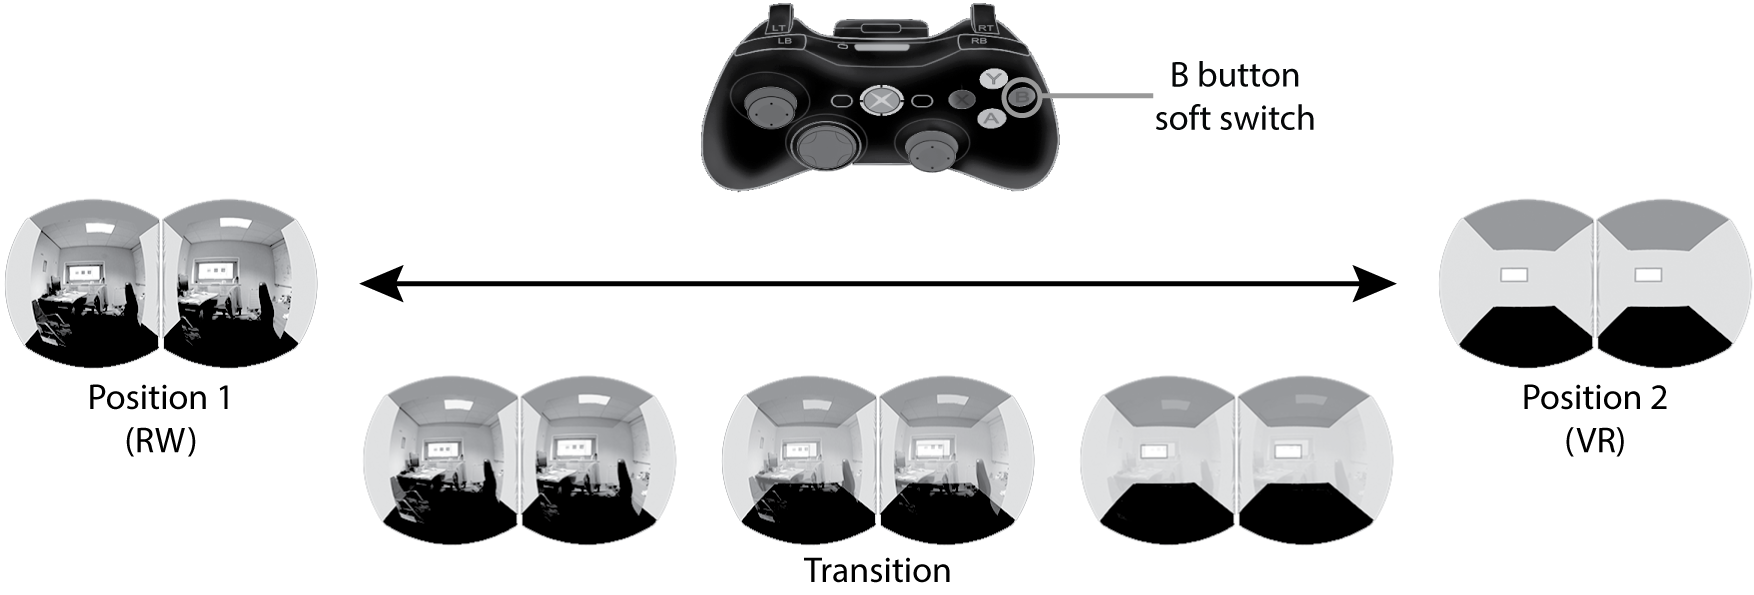
\includegraphics[width=\textwidth]{images/switching-soft-with-controller.png}
		\caption{Switch with linear interpolation.}
		\label{scenario12}
	\end{center}
\end{figure}

\subsubsection{Analogue selectable opacity}
The user pulls the right analogue trigger (\texttt{[RT]}) on the controller, where the position of the trigger maps directly to the opacity of the game objects that the webcam feeds are rendered upon. The user can choose to stop at any intermediary position that suits their needs, keeping the level of opacity of the webcam feeds at that position, as well as controlling the rate at which the visual stimuli from the RW environment fade (by changing how quickly they change their depression of the trigger). Pulling the trigger all the way in displays only visual stimuli from the VR environment, while releasing it completely displays only visual stimuli from the RW environment. The number of intermediary positions is limited only by the resolution of the trigger \& the encoding of the value.

This method allows the user to superimpose VR visual stimuli upon RW visual stimuli. This is similar, but not identical, to AR, as instead of displaying a small number of virtual objects upon the user's view of their RW environment, a complete VR environment is superimposed upon the user's view of their RW environment. Figure \ref{scenario2} illustrates this scenario.

\begin{figure}[h]
	\begin{center}
		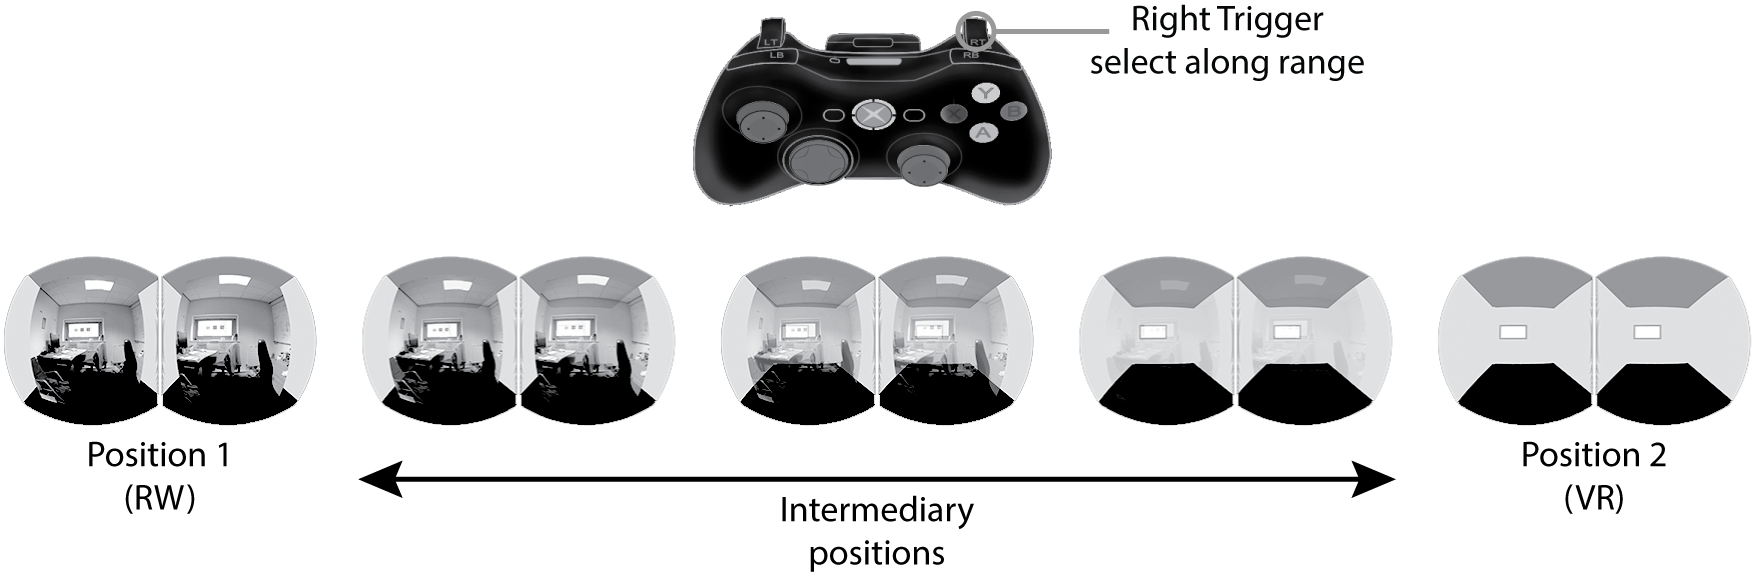
\includegraphics[width=.9\textwidth]{images/switching-analogue-with-controller.png}
		\caption{Analogue selectable opacity.}
		\label{scenario2}
	\end{center}
\end{figure}

\subsubsection{Periodic hard switches}
\label{subsub-periodic}
Independent or in addition to any of the previous scenarios, the visual stimuli displayed by the HMD switch from RW to VR at a set interval \& for a set amount of time. For example, every 3 seconds the stimuli switch from RW to VR for 0.2 of a second before switching back from VR to RW. Any user triggered transitions cause the interval timer to be reset, such that an `automated' switch will never occur after less time from a user triggered switch than the set interval. Automated transitions are disabled whilst \texttt{[RT]} is at all depressed. Figure \ref{scenariotimed} illustrates this scenario, where \texttt{i} represents the interval between switches \& \texttt{d} represents the duration of the switch from RW to VR.


\begin{figure}[h]
	\begin{center}
		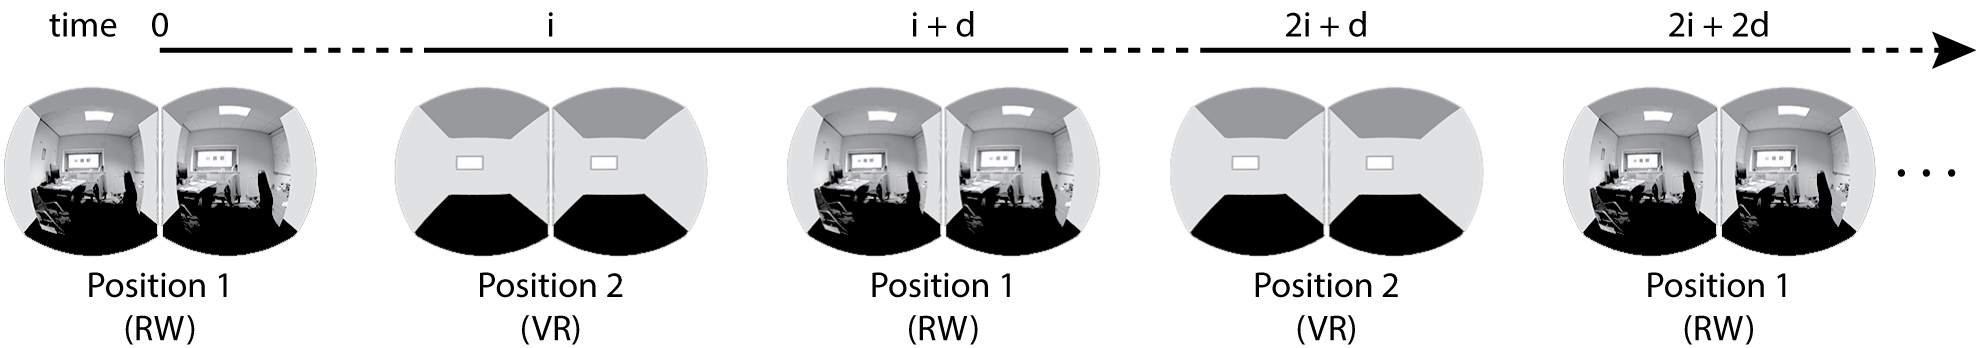
\includegraphics[width=\textwidth]{images/timed-switch.png}
		\caption{Periodic hard switches.}
		\label{scenariotimed}
	\end{center}
\end{figure}


\newpage

\subsubsection{Reduced maximum opacity}
\label{subsub-baseopacity}
Independent or in addition to any of the previous scenarios, the maximum opacity of the game objects that the webcam feeds are rendered upon is reduced, such that the `default' position at which a transition has not been triggered (either by a button press, trigger movement or by a periodic switch) displays VR superimposed upon RW. Figure \ref{scenariobaseopacity} illustrates this scenario in combination with a hard switch (from section \ref{sub-hardswitch}) in which the user triggers hard switches between the default position of a superimposition of VR upon RW \& a position where only VR stimuli are present.

\begin{figure}[h]
	\begin{center}
		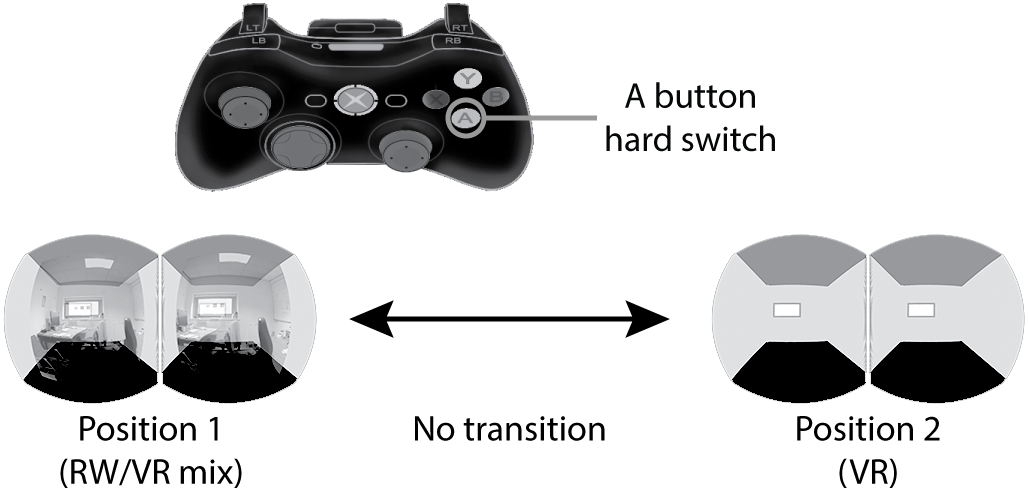
\includegraphics[width=0.7\textwidth]{images/base-opacity-hard-switch.png}
		\caption{Hard switch from reduced maximum opacity.}
		\label{scenariobaseopacity}
	\end{center}
\end{figure}

%=========================================================================================================
%=========================================================================================================

\subsection{Experimental Task \& Setting}
For these experiments, the HMD is worn upon the head of the participant \& is connected to the laptop computer, battery pack \& wireless receiver worn in a satchel. The smartphone is held in the left hand \& the Xbox controller is held in the right hand (all of the buttons \& triggers used for these experiments are on the right hand side of the controller, designed to be activated with only the right hand).

A task similar to that employed in the first investigation (see section \ref{investigation1} will be employed, encouraging participants to encounter multiple different scenarios of moving, remaining stationary, etc.


%=========================================================================================================


%\textit{Two different buildings have been prepared for use with the Mirrorshades platform, with VR environments constructed \& the IndoorAtlas IPS deployed. The first is a modern building accompanied by a VR environment that closely depicts it in the present day. The second is a historic building accompanied by a VR environment that differs markedly from the present day, by depicting its state a point hundreds of years in the past.}

%\textit{In the first, participants will be given a simple task to complete which will encourage them to engage with the VR environment even though it presents a similar view to their RW environment. In the second scenario, participants will be prompted to engage in more free form exploration of their environments, comparing \& contrasting the markedly different VR environment with what they see around them in their RW environment.}

%\subsection{Jack Cole Building}
%The School of Computer Science Jack Cole building at St Andrews is a modern building, built in 2004. The VR environment accompanying the building is a fairly close representation of the building as it stands today. Figure \ref{jc_layout} shows the layout of the building \& the path that IndoorAtlas has been prepared for.

%There are four coloured panels (red, green, blue \& yellow) situated within the VR building upon walls, floor \& ceiling. Participants will be asked to remember in what order these panels are seen as they walk a lap of the building. This task is designed to encourage participants to switch between RW \& VR visual stimuli, even though the VR visual stimuli are very similar to those of the RW environment. This scenario is also intended to encourage participants to keep moving, rather than stopping at \& starting.

%\begin{figure}[h]
%	\begin{center}
%		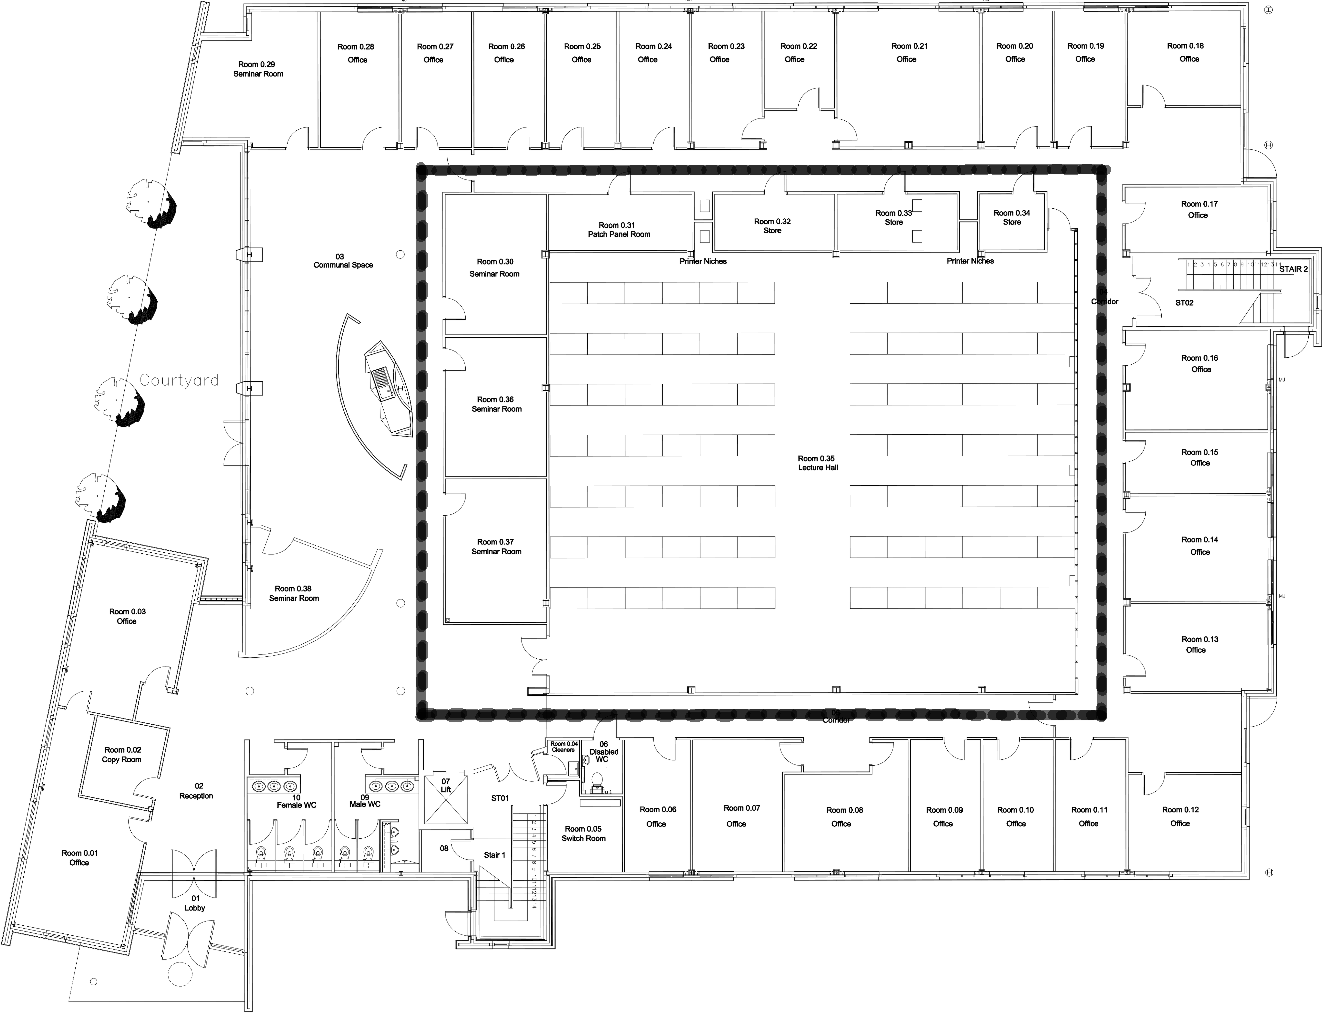
\includegraphics[width=0.7\textwidth]{images/JC_layout.png}
%		\caption{Floor plan of Jack Cole building, with IPS route.}
%		\label{jc_layout}
%	\end{center}
%\end{figure}

%=========================================================================================================
%=========================================================================================================

\subsection{Evaluation}
%*** explain why we need both Quantitative & Qualitative data?

%What transition styles are preferred in what situations?
%What affects which transition styles are preferred (eg what are the 'situations')?

Evaluating users' preferences toward different methods of transitioning between visual stimuli in different situations pertains to studying their reactions \& responses to ascertain the effect upon their focus of attention, concepts which are largely psychological in nature \& highly subjective~\cite{Ijsselsteijn2001}. Thus, subjective measures will produce the bulk of the data for evaluation. However, objective data will also be collected \& cross referenced with the subjective data in attempts to support or contradict any relationships that are identified.

It is hypothesized that a manner of transitioning between visual stimuli which results in a less severe BIP will be preferable to a manner of transitioning which results in a worse BIP. As focus in the Waterworth model is most closely related to presence in the VR literature~\cite{Waterworth2001}, one of the subjective measures that will be used in this evaluation will be an established presence measure, to try to capture the behaviour of the user's position upon the focus axis.

\subsubsection{Subjective Quantitative - Post-Task Questionnaire}
After completing the task, participants will respond to the Igroup Presence Questionnaire (IPQ)~\cite{Schubert2001} (see appendix \ref{ipqitems} for the items of the IPQ) which will provide subjective quantitative insight into their experiences with the system, in particular in relation to their position upon the focus axis of the combined model. The IPQ represents a useful questionnaire for evaluation of users' subjective experiences of using the Mirrorshades platform because its terms, especially in the `spatial involvement' scale, question about the RW environment in a manner that does not explicitly present it as a `distraction' from the VR interaction as many other presence questionnaires do.
%examples of other presence questionnaires that present RW stimuli as 'distractions'?

%citation for the components being independent
%The IPQ consists of one general item (G), five items in the `spatial presence' (SP) scale, four items in the `involvement' scale (INV) \& four items in the `realness' scale (REAL). For the purposes of this study, all of the REAL items save REAL2 will be omitted from the questionnaire. The REAL items are primarily concerned with eliciting how `real' participants considered the virtual environment to be. These questions are useful for traditional VR experiences where the user is encouraged to suspend belief \& believe the VR environment they are perceiving to be `real' (the same experiences for which RW stimuli are usually considered a `distraction'). The Mirrorshades platform, however, is less concerned with convincing participants that a VR environment is real \& is more concerned with the juxtaposition of VR \& RW environments.
%It is believed that the other REAL questions will get the participants thinking about the wrong things & hamper their responses when talking about XR

%hypothesis
Whilst a traditional VR experience would hope to elicit high SP1 \& SP4 results combined with low INV1 \& INV3 results, Mirrorshades participants are expected to report high SP1 \& SP4 combined with \textit{high} INV1 \& INV3. The results from participants in this investigation will be compared against those who partook in a `traditional' VR experience wherein RW stimuli were considered a distraction.

% *** But what about the factor analysis, what effect does removing the REAL component have on that?

\subsubsection{Subjective Qualitative - Interview}
A structured interview will be performed after the IPQ has been completed.

\subsubsection{Objective Quantitative - Automatic Data Logging}
The Unity app logs the following quantitative data each frame to a tab separated variable (\texttt{.tsv}) file;

\begin{itemize}
	\item \texttt{<frame number>}
	\item \texttt{<timestamp>} - according to the laptop's internal clock
	\item \texttt{<original\_position>} - the position as a Unity \texttt{Vector3} where the user begins the experiment
	\item \texttt{<position>} - the position as a Unity \texttt{Vector3} where the user is on this frame
	\item \texttt{<delta\_x>} \& \texttt{<delta\_z>} - the difference in the \texttt{x} \& \texttt{z} axes between \texttt{<original\_position>} \& \texttt{<position>} on this frame
	\item \texttt{<left\_rotation>} \& \texttt{<right\_rotation>} - the orientations as Unity \texttt{Quaternion} of the two Unity camera game objects
	\item \texttt{<base\_oapcity>} - the maximum opacity of the game objects upon which the webcam feeds are rendered (see section \ref{subsub-baseopacity})
	\item \texttt{<left\_opacity>} \& \texttt{<right\_opacity>} - the opacity on this frame of the game objects upon which the webcam feeds are rendered
	\item \texttt{<auto\_tick>} - whether a periodic switch is in progress (see section \ref{subsub-periodic})
	\item \texttt{<auto\_duration>} \& \texttt{<auto\_spacing>} - the interval \& duration values of the periodic hard switching
	\item \texttt{<framerate>} - an estimate of the current frame rate (frames per second)
	\item \texttt{<A\_button>}, \texttt{<B\_button>} \& \texttt{<right\_trigger>} - the current values of these inputs on the controller
\end{itemize}

\vspace{4mm}

An example line of this output;

\begin{center}
	\texttt{420	08-05-2014 12-34-36-257	(3.4, 1.0, -8.3)	(0.3, 1.0, -8.3)	3.153522	0.0001955032	(-0.1, -0.7, -0.1, 0.7)	(-0.1, -0.7, -0.1, 0.7)	1	1	1	False	0	0	39.57977	False	False	0}
\end{center}

These data are expected to reveal relationships between various different metrics \& the choice of transition methods. For example, it is expected that participants will perform short transitions to VR or transitions to a mix of RW \& VR when moving \& perform longer transitions to VR when stationary. This kind of relationship will support or contradict the subjective data collected through questionnaire \& interview.

%*** SUS?

\subsubsection{Objective Qualitative - Video Recording}
%*** talk about not prompting them with 'think aloud' vs prompting (where prompting changes their responses)
During experiments, the video feed being displayed by the HMD will be recorded \& the user will be recorded using a video camera (both video \& audio). The video of the HMD graphics will be used in comparison with the quantitative data, while the video \& audio recording of the user will provide objective insight into their behaviour.

%\subsection{Evaluation Techniques}
%These data will make it possible both to statistically assess preferred switching/fading methods, but also to infer any relationships between different switching/fading methods \& other behaviours: for example, a certain style of switching/fading may frequently appear after a period of movement, but rarely when the participant is stationary.

%\section{Hypothesis}
%Null hypothesis includes things like;
%\begin{itemize}
%	\item different transitions do not alter user `enjoyment'
%	\item users will not prefer one transition over another
%	\item choice of transition will have no effect on circumstances/scenarios
%	\item users will not move head less when walking
%	\item users will not spend less time in virtual when walking
%	\item etc.
%\end{itemize}